\documentclass[a4paper,12pt]{extarticle}
\usepackage[table,xcdraw]{xcolor}
\usepackage{pgfplots}
\usepackage[unicode, pdftex]{hyperref}
\usepackage[T2A]{fontenc}
\usepackage[utf8]{inputenc}
\usepackage[english,russian]{babel}
\usepackage{amsmath,amsfonts,amsthm, mathtools}
\usepackage{amssymb}
\usepackage{graphicx}
\graphicspath{{images/}}
\usepackage{wrapfig}
\usepackage{floatrow}
\usepackage{setspace}
\usepackage[headings]{fancyhdr}
\usepackage[margin=10pt,font={small,stretch=0,9},labelfont=bf,labelsep=period,
justification=centerlast]{caption}
\usepackage{array,tabularx,tabulary,booktabs}
\RequirePackage{multirow}
\RequirePackage{multicol}
\RequirePackage{longtable}
\usepackage{indentfirst}
\usepackage{hyperref}
\usepackage{icomma}
\newcommand*{\hm}[1]{#1\nobreak\discretionary{}
	{\hbox{$\mathsurround=0pt #1$}}{}}
\usepackage{soulutf8} 
\usepackage{etoolbox} 
\usepackage{geometry}
\geometry{top=20mm}
\geometry{bottom=20mm}
\geometry{left=20mm}
\geometry{right=20mm}
\DeclareMathOperator{\sgn}{\mathop{sgn}}
\usepackage[OT1]{fontenc}
\usepackage{amsmath}
\usepackage{amsfonts}
\usepackage{amssymb}
\usepackage{wasysym}
\usepackage{wrapfig}
\usepackage{physics}
\usepackage[normalem]{ulem}
\graphicspath{{pictures/}}
\DeclareGraphicsExtensions{.png,.jpg,.jpeg}
\usepackage{indentfirst}
\usepackage[T2A]{fontenc}
\usepackage{subfigure}
\usepackage{fancyhdr}
\usepackage{caption}

\usepackage{tabularx}
\usepackage{floatrow}
\usepackage{multicol}
\usepackage{lastpage}

\pgfplotsset{
  MyStyle1/.style={
    axis lines = middle,
    enlargelimits = true,
    grid=both,
    grid style={line width=.1pt, draw=gray!10},
    major grid style={line width=.2pt,draw=gray!50},
    minor tick num=5,
    enlargelimits=0.05,
    ticklabel style={font=\tiny,fill=white},
    xlabel style={at={(ticklabel* cs:1)},anchor=north west},
    ylabel style={at={(ticklabel* cs:1)},anchor=south east},
  }
}
\def\Slope{1.5}
\def\Intercept{-20}


% Настройка отчёркиваний и нумерации
\usepackage{fancyhdr}
\pagestyle{fancy}
\fancyhf{}

\fancyhead[L]{\nouppercase{\leftmark\hfill}}
\fancyfoot[RO, RE]{Страница \thepage \ из \pageref{LastPage}}
\renewcommand{\headrulewidth}{0.5pt}
\renewcommand{\footrulewidth}{0.5pt}

\usepackage{titlesec}
\titlelabel{\thetitle.\quad}

\pgfplotsset{compat=1.18}
\begin{document}

\thispagestyle{empty}
\begin{center}
	\textit{Федеральное государственное автономное образовательное\\ учреждение высшего образования }
	
	\vspace{0.5ex}
	
	\textbf{«Московский физико-технический институт\\ (национальный исследовательский университет)»}
\end{center}

\vspace{10ex}
\begin{figure}[!h]
  \begin{center}
    
\includegraphics[width = 0.8\textwidth]{MIPT.png}
  \end{center}
\end{figure}

\begin{center}
	
	\textbf{Лабораторная работа № 4.3.6}
	
	\vspace{1ex}
	
	по курсу общей физики
	
	на тему:
	
	\textbf{\textit{<<Дифракция света на периодических
структурах (саморепродукция)>>}}
	
	\vspace{20ex}
	
	\begin{flushright}
		\noindent
		\textit{Работу выполнил:}\\  
		\textit{Легких Никита \\(группа Б05-301)}
	\end{flushright}
	\vfill
	Долгопрудный \\ \today
	\setcounter{page}{1}
\end{center}
\newpage

% Конец шаблона
\newpage

\textbf{Цель работы:} Изучение явления саморепродукции и применение его
к измерению параметров периодических структур. \\ \\
\textbf{В работе используются:} лазер самоделка (длина волны $\lambda = 532$ нм), кассета с сетками, мира, короткофокусная линза с микрометрическим винтом, экран, линейка.
\section*{Теоретическая справка} 
При дифракции плоской световой волны на предмете с периодической структурой наблюдается следующее явление: на некотором расстоянии от предмета вдоль направления распространения волны появляется его изображение, периодически повторяющееся при дальнейшем движении вдоль той же оси. Это явление называется \textit{явлением саморепродукции}.

Запишем выражение для комплексной амплитуды волны, прошедшей через периодическую решётку, в плоскости, отстоящей на расстоянии $z$ от плоскости решётки:
\begin{equation*}
    f(x, z) = \sum c_ne^{i(u_nx + \sqrt{k^2-u_n^2}z)}.
\end{equation*}
Фаза $n$-ой плоской волны плоской волны в плоскости $z = \text{const}$ равна $\varphi_n = \sqrt{k^2 - u_n^2}z\approx kz - \frac{zu_n^2}{2k}$. Сравним набег фазы $n$-ой плоской волны с набегом фазы $\varphi_0$ плоской волны, бегущей вдоль оси $z$: $\varphi_0 = kz$. Получаем разность фаз
\begin{equation}\label{dphi}
    \Delta\varphi_n = \varphi_n - \varphi_0 = \frac{z}{2k}\left(\frac{2\pi}{d}\right)^2n^2 = \pi\frac{\lambda z}{d^2}n^2.
\end{equation}

Рассмотрим плоскость наблюдения, отстоящую от плоскости решётки на расстояние $z_m$, при 
\begin{equation}\label{ZZZ}
    z_m = m\frac{2d^2}{\lambda},\quad z\in\mathbb{N}.
\end{equation}
В этой плоскости из \eqref{dphi} имеем разность $\Delta\varphi_n = 2\pi m n^2$. Получаем, что разность фаз кратна $2\pi$ при любых целых $n$. Аналогично, разность фаз между любыми двумя волнами кратна $2\pi$: $\Delta\varphi_{ij} = 2\pi m(i^2-j^2)$. Получается, что фазовые соотношения между слагаемыми плоскими волнами одинаковы в плоскости решётки и в плоскости наблюдения, откуда следует, что результат интерференции этих волн также одинаков. В этом и заключается суть эффекта саморепродукции.

\section*{Установка}
\begin{figure}[h]
    \centering
    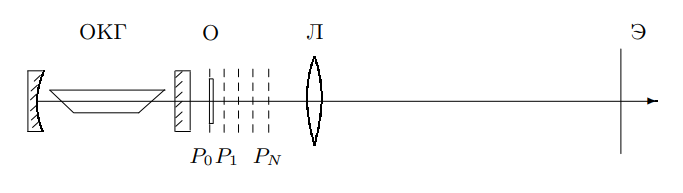
\includegraphics[width=0.6\textwidth]{pics/setup.png}
    \caption{Схема установки для наблюдения саморепродукции/дифракции}
    \label{fig:setup}
\end{figure}

Хорошим приближением плоской волны в нашем эксперименте служит излучение лазера. Схема экспериментальной установки показана на рис. \ref{fig:setup}. Луч гелий-неонового лазера из генератора оптического квантового генератора (ОКГ) направляется на периодическую структуру О в плоскости $P_0$. В качестве  В плоскостях $P_1$-$P_N$ возникают изображения объекта, которые с помощью линзы Л можно поочерёдно проецировать на экран, установленный в плоскости Э.

Если убрать линзу, то на экране наблюдается картина дифракции луча лазера на периодическом объекты. Экран устанавливается достаточно далеко от объекта, так что лучи, соответствующие различным порядкам дифракции ($\sin \theta_n = n\lambda/d$), разделяются. Измеряя расстояние между дифракционными максимумами, можно определить $\sin \theta_n$ и $d$.

В качестве периодических структур в данной работе используется мира~--- набор различным образом ориентированных одномерных решёток разного период, а также набор из пяти двумерных сеток-решёток. Последние можно рассматривать как пары взаимно перпендикулярных решёток.

\section*{Задание}
{\large \textbf{A Исследование двумерных решёток}}\\ \\ 
\textbf{\uppercase\expandafter{\romannumeral 1} Определение периода решёток по их пространственному спектру}\\ 



\begin{minipage}[]{0.45\textwidth} 
    Включаем лазер, подставляем решетки. 
    
    Для каждой решетки кассеты получаем следующие измерения: 

    Здесь ось X - горизонтальная ось с нулем в главном максимуме, ось Y - вертикальная ось с нулем там же, все расстояния представлены в сантиметрах.

    В качестве погрешности данных измерений берем 0.1 см, 0.5 см - приборная погрешность (обычная железная линейка), ещё 0.5 см берем как измерительную погрешность.

    Расстояние до экрана $L = (136\pm0.5)$ см, большая погрешность обуслена необходимостью использования дополнительной линейки и неточностью определения положения решетки.
\end{minipage}%
\hfill 
\begin{minipage}[t]{0.45\textwidth} 
   \begin{tabular}{|cccc|}
        \hline
        \multicolumn{1}{|c|}{X}  & \multicolumn{1}{c|}{Y}  & \multicolumn{1}{c|}{Расстояние X} & Расстояние Y \\ \hline
        \multicolumn{4}{|c|}{1 кассета}                                                                       \\ \hline
        \multicolumn{1}{|c|}{4}  & \multicolumn{1}{c|}{0}  & \multicolumn{1}{c|}{10.9}         & 0            \\ \hline
        \multicolumn{1}{|c|}{-4} & \multicolumn{1}{c|}{0}  & \multicolumn{1}{c|}{-10.9}        & 0            \\ \hline
        \multicolumn{4}{|c|}{2 кассета}                                                                       \\ \hline
        \multicolumn{1}{|c|}{0}  & \multicolumn{1}{c|}{4}  & \multicolumn{1}{c|}{0}            & 9.6          \\ \hline
        \multicolumn{1}{|c|}{0}  & \multicolumn{1}{c|}{-3} & \multicolumn{1}{c|}{0}            & 7.2          \\ \hline
        \multicolumn{4}{|c|}{3 кассета}                                                                       \\ \hline
        \multicolumn{1}{|c|}{-8} & \multicolumn{1}{c|}{0}  & \multicolumn{1}{c|}{-9.7}         & 0            \\ \hline
        \multicolumn{1}{|c|}{8}  & \multicolumn{1}{c|}{0}  & \multicolumn{1}{c|}{9.7}          & 0            \\ \hline
        \multicolumn{4}{|c|}{4 кассета}                                                                       \\ \hline
        \multicolumn{1}{|c|}{8}  & \multicolumn{1}{c|}{0}  & \multicolumn{1}{c|}{4.8}          & 0            \\ \hline
        \multicolumn{1}{|c|}{0}  & \multicolumn{1}{c|}{8}  & \multicolumn{1}{c|}{0}            & 4.7          \\ \hline
        \multicolumn{4}{|c|}{5 кассета}                                                                       \\ \hline
        \multicolumn{1}{|c|}{8}  & \multicolumn{1}{c|}{0}  & \multicolumn{1}{c|}{3.7}          & 0            \\ \hline
        \multicolumn{1}{|c|}{0}  & \multicolumn{1}{c|}{8}  & \multicolumn{1}{c|}{0}            & 3.6          \\ \hline
    \end{tabular}   
\end{minipage}
\\ \\ 
\textbf{\uppercase\expandafter{\romannumeral 2} Определение периода решёток по изображению, увеличенному с помощью линзы}\\ 

Установим короткофокусную линзу на небольшом расстоянии от лазера,
между ней и лазером установим кассету с сетками, настроим систему так,
чтобы было видно резкое изображение проволочки(т.е. непериодического
объекта). Определим размеры $D$ клеток на экране для всех сеток, для
которых это возможно (в нашем случае это сетки 3, 4 и 5). Полученные
результаты внесём в таблицу:\\
\begin{tabular}{|c|c|c|c|c|}
\hline
номер кассеты & $X$, см   & $n$  & $D$, см  & $\Delta D$, см   \\ \hline
5  & 5.6 & 14 & 0.40 & 0.01  \\ \hline
4  & 4.9 & 16 & 0.31 & 0.01  \\ \hline
3  & 2.5 & 17 & 0.15 & 0.01  \\ \hline
\end{tabular} \\
Не забудем измерить расстояния до линзы и экрана: $a = (5.2\pm0.3)$ см, $b = (129.5\pm0.5)$
\newpage

\textbf{\uppercase\expandafter{\romannumeral 3} Исследование эффекта саморепродукции с помощью сеток}\\ 
К сожалению в моем случае удалось измерить лишь 1.5 кассеты, то есть полноценные измерения у мен есть только для 5 кассеты, то есть для самой мелкой. Сами измерения представлены ниже: \\
\begin{tabular}{|ccccc|}
\hline
\multicolumn{5}{|c|}{5 кассета}                                                                                        \\ \hline
\multicolumn{1}{|c|}{$N$} & \multicolumn{1}{c|}{0}     & \multicolumn{1}{c|}{1}     & \multicolumn{1}{c|}{2}     & -1    \\ \hline
\multicolumn{1}{|c|}{$z$, см} & \multicolumn{1}{c|}{3,325} & \multicolumn{1}{c|}{4,355} & \multicolumn{1}{c|}{5,220} & 1,460 \\ \hline
\multicolumn{5}{|c|}{4 кассета}                                                                                        \\ \hline
\multicolumn{1}{|c|}{$N$} & \multicolumn{1}{c|}{0}     & \multicolumn{1}{c|}{1}     & \multicolumn{1}{c|}{-}     & -     \\ \hline
\multicolumn{1}{|c|}{$z$, см} & \multicolumn{1}{c|}{3,325} & \multicolumn{1}{c|}{5,835} & \multicolumn{1}{c|}{-}     & -     \\ \hline
\end{tabular} \\ \\

{\large \textbf{Б Исследование решёток миры}}\\ \\ 
Установим миру на место кассеты и проведем аналогичные вычисления для элементов миры под номером 20 и 25.\\
Расстояние от линзы до миры $a = (5,5 \pm 0,1)$ см, расстояние от линзы до экрана $b = (128,5 \pm 0,5)$ см. Следовательно, расстояние от миры до экрана равно $L = (134,0 \pm 0,5)$ cм.\\
Настроим систему так, чтобы было видно резкое изображение, и, вычислив значение $D$ в этом положении, получим значение $d_\text{л}$.\\
Также построим график зависимости $z_N = f(N)$, где $z_N$ - координаты на нониусной шкале плоскостей саморепродукции.\\
И в конце, убрав линзу и вычислив расстояние между максимумами, определим $d_\text{сп}$.\\
\begin{figure}[!h]
    \begin{minipage}[]{0.49\textwidth} 
        
\includegraphics[width=1\textwidth]{pics/4.png}
        \caption{График $z(n)$ для элемента миры №25 и №20}
    \end{minipage}%
    \hfill 
    \begin{minipage}[]{0.49\textwidth} 
        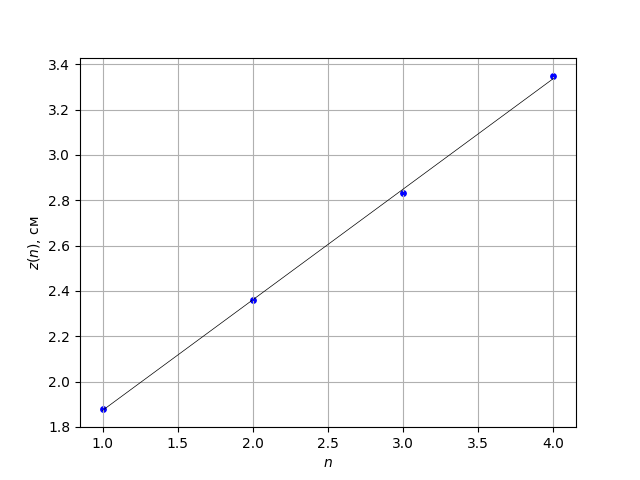
\includegraphics[width=1\textwidth]{pics/5.png}
    \end{minipage}
\end{figure}

{\large \textbf{В Обработка данных}}\\ \\ 
1) Сначала определим $d_{\text{сп}}$, используя соотношение $\sin \theta \approx \theta \approx \frac{x}{L}$, но перед тем как его использовать надо определить  погрешность использования данного соотношения: \\
Возьмем харатерные для данного эксперимента отклонения $x \approx 4$ см и $L \approx 130$ см, для этих значений: $$\epsilon = 2 \frac{\sin \theta - x/L}{\sin \theta + x/L} \cdot 100\% \approx 0.05 \%,$$ что есть сильно меньше остальных погрешностей эксперимента. Тогда  $d_{\text{сп}} = \frac{\lambda L }{X}$ (или Y).

В случае же использования линзы мы пользуемся тем же соотношением но с поправкой на увеличенное изображение и итого получаем итоговую формулу: $d_{\text{лз}} = \frac{D a}{b}$. 

Для исследования по репродукциям пользуемся соотношением $z_m = m \cdot \frac{2d^2}{\lambda} \Rightarrow d = \sqrt{\frac{\lambda k}{2}},$ где $k$ - угловой коефициент соответствующего графика. Сначала построим требуемые зависимости, потом уже будем считать $k$: 
\begin{figure}[!h]
    \begin{minipage}[]{0.49\textwidth} 
        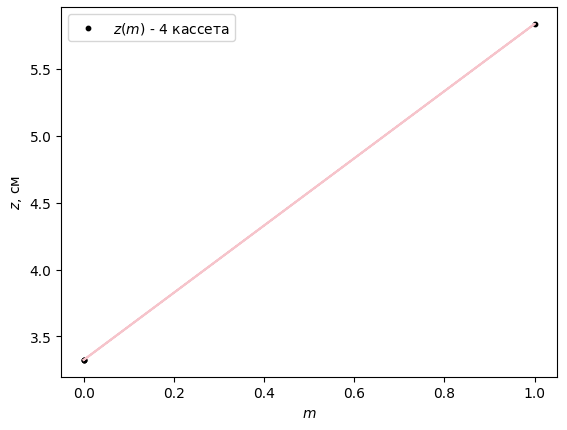
\includegraphics[width=1\textwidth]{pics/4 кассета.png}
        \caption{График $z(n)$ для элемента миры №25 и №20}
    \end{minipage}%
    \hfill 
    \begin{minipage}[]{0.49\textwidth} 
        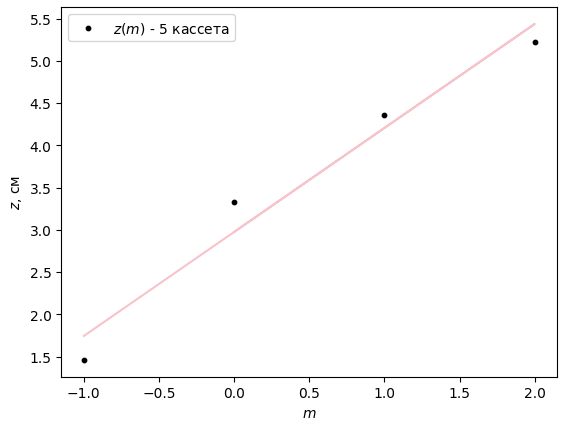
\includegraphics[width=1\textwidth]{pics/5 кассета.png}
    \end{minipage}
\end{figure}\\
Используемые формулы: $k_4 = \frac{y_2 - y_1}{x_2 - x_1} \Rightarrow \Delta k_4 = 2\epsilon_z \cdot k_4$, $\Delta z_{\text{репр}} = 0.01$ см, последняя погрешность следует из точности измерения нониусом; $k_5$ определяем по МНК. 
\begin{equation}
\left\{
\begin{aligned}
    k_4 = (2.51\pm0.02), \text{см}\\
    \frac{\delta k_4}{k_4} = 0.6 \%
\end{aligned}
\right.
\end{equation}
\begin{equation}
\left\{
\begin{aligned}
    k_5 = (1.23\pm0.2), \text{cм}\\
    \frac{\delta k_5}{k_5} = 10 \%
\end{aligned}
\right.
\end{equation}
Пересчитываем полученные значения и сводим их в одну таблицу:
\begin{table}[H]
\centering
\begin{tabular}{|c|c|c|c|c|c|c|}
\hline
№ сетки & $d_\text{сп}$, мм & $\sigma_{d_\text{сп}}$, мм & $d_\text{л}$, мм & $\sigma_{d_\text{л}}$, мм & $d_\text{реп}$, мм & $\sigma_{d_\text{реп}}$, мм \\ \hline
1 & 0,02015 & 0,0002 & \multicolumn{4}{|c|}{-} \\ \hline
2 & 0,0315 & 0,0003 & \multicolumn{4}{|c|}{-} \\ \hline
3 & 0,0605 & 0,0003 & 0,065 & 0,003 & \multicolumn{2}{|c|}{-}  \\ \hline
4 & 0,1186 & 0,0013 & 0,126 & 0,004 & 0,092 & 0,002 \\ \hline
5 & 0,1580 & 0,0030 & 0,168 & 0,005 & 0,160 & 0,007 \\ \hline
\end{tabular}
\caption{Сводная таблица результатов для сеток}
\end{table}
Для миры же получаем: 
\begin{table}[H]
\begin{tabular}{|c|c|c|c|c|c|c|}
\hline
№ элемента & $d_\text{сп}$, мкм & $\sigma_{d_\text{сп}}$, мм & $d_\text{л}$, мм & $\sigma_{d_\text{л}}$, мм & $d_\text{реп}$, мм & $\sigma_{d_\text{реп}}$, мм \\ \hline
25 & 0,04446 & 0,00022 & 0,0432 & 0,0023 & 0,033 & 0,017 \\ \hline
20 & 0,0594 & 0,0004 & 0,060 & 0,003 & 0,0360 &	0,0006 \\ \hline
\end{tabular}
\caption{Сводная таблица результатов для миры}
\end{table}
Анализируя полученные значения, можно заметить, что дополнительные методы измерения дали совпадающие с хорошей степенью точности, однако результаты метода, основанного на эффекте саморепродукции, сходятся с остальными по порядку, но с точностью до коэффициента.\\
Таким образом, можно сделать вывод, что исследуемый в данной работе метод, основанный на явлении саморепродукции, позволил довольно точно оценить порядку величин параметров решёток, однако наиболее точным оказался метод измерения пространственного спектра.\\
Также нам не удалось с помощью нашей установки исследовать 1-3 кассеты с помощью метода репродукции.
\end{document}